\documentclass[10pt,twocolumn,letterpaper]{article}

\usepackage{cvpr}
\usepackage{times}
\usepackage{epsfig}
\usepackage{graphicx}
\usepackage{amsmath}
\usepackage{amssymb}

% Include other packages here, before hyperref.

% If you comment hyperref and then uncomment it, you should delete
% egpaper.aux before re-running latex.  (Or just hit 'q' on the first latex
% run, let it finish, and you should be clear).
\usepackage[breaklinks=true,bookmarks=false]{hyperref}

\cvprfinalcopy % *** Uncomment this line for the final submission

\def\cvprPaperID{****} % *** Enter the CVPR Paper ID here
\def\httilde{\mbox{\tt\raisebox{-.5ex}{\symbol{126}}}}

% Pages are numbered in submission mode, and unnumbered in camera-ready
%\ifcvprfinal\pagestyle{empty}\fi
\setcounter{page}{1}
\begin{document}

%%%%%%%%% TITLE
\title{Free-hand Sketch Recognition Classification}

\author{Wayne Lu\\
Stanford University \\
{\tt\small waynelu@stanford.edu}
% For a paper whose authors are all at the same institution,
% omit the following lines up until the closing ``}''.
% Additional authors and addresses can be added with ``\and'',
% just like the second author.
% To save space, use either the email address or home page, not both
\and
Elizabeth Tran\\
Stanford University\\
{\tt\small eliztran@stanford.edu}
}

\maketitle
%\thispagestyle{empty}

%%%%%%%%% ABSTRACT
\begin{abstract}

People use sketches to express and record their ideas. Free-hand sketches are usually drawn by non-artists using touch sensitive devices rather than purpose-made equipments; thus, making them often highly abstract and exhibit large intraclass deformations. This makes automatic recognition of sketches more challenging than other areas of image classification because sketches of the same object can vary based on artistic style and drawing ability. In addition, sketches are less detailed and thus harder to distinguish than photographs. Using a publicly available dataset of 20,000 sketches across 250 classes from Eitz et al. ~\cite{eitz2012hdhso}, we are applying ConvNets (CNNs) in order to improve performance to increase the recognition accuracy on sketches drawn by different people. In our experiments, we analyze the effects of several hyperparmeters on overall performance using a Residual Network (ResNet) approach.  
 
\end{abstract}

%%%%%%%%% BODY TEXT
\section{Introduction}
Sketching is one of the primary methods people use to communicate visual information. Since the era of primitive cave paintings, humans have used simple illustrations to represent real-world objects and concepts. Sketches are often abstract and stylized, varying based on artistic ability and style. In addition, sketches emphasize defining characteristics of real-world objects and ignore features which are either less important or more difficult to draw. For example, texture is almost never rendered unless it is important for recognition, such as the spikes on a hedgehog. In this way, sketches can be interpreted as a distillation of human visual recognition schemas.\

Sketch recognition attempts to recognize the intent of the user while allowing the user to draw in an unconstrained manner. This allows for the user to not have to spend time being trained how to draw on the system, nor will the system need to be trained on how to recognize each users particular drawing style. Deciphering freehand sketches can be viewed under the lens of image category recognition, a well studied problem in the computer vision community.  

However, the sketch recognition problem differs from traditional photographic image classification. First, sketches are less visually complex than photographs. Whereas color photographs have three color channels per pixel, sketches are encoded as either black-and-white or grayscale. Photographs contain visual information throughout the image whereas sketches consist primarily of blank space. Second, sketches and photographs have different sources of intraclass variation. Whereas photographic image classification faces obstacles such as camera angle, occlusion, and illumination, photographs are still grounded in reality. On the other hand, sketches differ based on artistic style, which is unique to every artist. While people can agree on what an object looks like, how they ultimately render the object can vary significantly.\

In this paper, we explore the use of deep convolutional neural networks (DCNN) architectures for sketch recognition. Since DCNNs are primiarly designed for photos, we demonstrate that DCNNs can be used for sketches, but there needs to be some modifications. Here, we are going to modify the ResNet architecture in order for it used for sketches. To the best of our knowledge, ResNets have not been utilized for online sketch recognition.\


%-------------------------------------------------------------------------
\section{Related Work}

Since SketchPad ~\cite{sutherland1964sketchpad}, sketch recognition has introduced sketching as a means of human computer interaction. Computer vision has since tried different approaches to achieve better results in multiple application areas. Eitz et al. ~\cite{eitz2012hdhso} was able to demonstrate classification rates can be achieved for computational sketch recognition by using local feature vectors, bag of features sketch representation and SVMs to classify sketches. Schneider et al.~\cite{schneider2014sketch} then modified the benchmark proposed by Eitz et al ~\cite{eitz2012hdhso}  by making it more focused on how the image should like, rather than the original drawing intention, and they also used SIFT, GMM based on Fisher vector encoding, and SVMs to achieve sketch recognition.\

Pervious work on sketch recognition generally extracts hand crafted features from the sketch followed by feeding them to a classifier.  Convolutional neural networks (CNN) have emerged as a powerful framework for feature representation and recognition ~\cite{krizhevsky2012imagenet}.  Convolutional neural networks are a type of neurobiologically inspired feed-forward artificial neural network which consist of multiple layers of neurons,  and  the neurons in each layer are then collected into sets. At the input layer, where the data gets introduce to the CNN, these neuron sets map to small regions of input image. Deeper layers of the network can be composed of local or global pooling (fully-connected) layers which combine outputs of the neuron sets from previous layer. The pooling is typically achieved through convolution-like operations. Deep neural networks (DNN), especially CNNs, can automatically learn features instead of manually extracting features and its multi layers learning can get more effective expression. When it comes to CNN design, the trend in the past few years has pointed in one direction: deeper networks [ ~\cite{krizhevsky2012imagenet}]. This move towards deeper networks  has been beneficial for many applications. The most prominent application has been object classification, where the deeper the neural network, the better the performance. However, current existing CNNs are designed for photos, and they are trained on a large amount of data to avoid overfitting.  \

CNNs, despite of having better classification performance, are harder to train, and an effective way to solve this problem is suggested using a ResNets [~\cite{hekaming2016}].  In a traditional activation layer, when the signal is sent backwards, the gradient must pass through all their convolutional layers, which can cause trouble due to the nonlinearities which are involved. ResNet, on the other hand, provides the networks with shortcut at each layer to make sending the gradient signal backwards more smoothly without the intermediate layers being diminished This shortcut allows addressing the problem of vanishing gradients and faster training. An example of a ResNet building block can be seen in Figure 1.\

 \begin{figure}[h]
	\begin{center}
	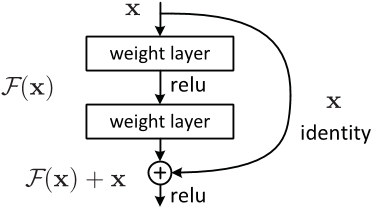
\includegraphics[width=.5\linewidth]{resnet}
	\caption{Model of a basic residual unit [ ~\cite{hekaming2016 }] }
	\end{center}
\end{figure}

Sketches, on the other hand, require special model architectures. In 2012, Eitz et al.~\cite{eitz2012hdhso} released the largest sketch object dataset. Since its release, a number of approaches have been proposed to recognize freehand sketches.  In Yu et al. ~\cite{yu2016sketch}, they proposed Sketch-a-Net, a different type of CNN that is customizable towards sketches. While Sarvadevabhatla et al. ~\cite{sarvadevabhatla2015freehand} used two popular ConvNets (ImageNet and a modified LeNet) to fine-tuned their parameters on the TU-Berlin sketch dataset in order to extract deep features from CNNs to recognize hand-drawn sketches. The current state-of-the-art is [~\cite{seddati2016deepsketch}], where propose a ConvNet for classification but they also include in feature extraction and similarity search. 


%-------------------------------------------------------------------------

\section{Method}

The ResNet model introduced in [~\cite{hekaming2016}] is our starting point for the network design.  ResNet  is specifically designed for images in ImageNet and accepts images with size 256 � 256 and classifies them in 1000 categories. However, since ResNet is used for images and we are trying to classify sketches, we did some customization to the original network. We chose to use this ResNet architecture in order to improve performance over traditional multi-class support vector classification.  \
 
 Tensorflow is a scientific open source computing framework with wide support for neural network implementations.  For our framework, we used Tensorflow to implement and train different insipiried ResNet Models. \\
 

\begin{figure}[h]
\begin{center}
\begin{tabular}{l | l | l}
Layer & Output Size & Feature Depth \\ \hline \hline
Input	& 128x128x1\\
Dropout &128x128x1 \\
7x7 conv, 64, /2	 & 64x64x64\\
3x3 residual unit, 64	& 64x64x64\\
3x3 residual unit, 64 & 64x64x64\\
3x3 residual unit, 64	& 64x64x64\\
Dropout	& 64x64x64 \\
3x3 residual unit, 128, /2 & 32x32x128\\
3x3 residual unit, 128 & 32x32x128\\
3x3 residual unit, 128 &	32x32x128\\
Dropout & 32x32x128\\
3x3 residual unit, 256, /2 & 16x16x256\\
3x3 residual unit, 256 & 16x16x256\\
3x3 residual unit 256	 & 16x16x256\\
Dropout	& 16x16x256\\
3x3 residual unit, 512, /2	& 8x8x512\\
3x3 residual unit, 512	& 8x8x512\\
3x3 residual unit, 512& 	8x8x512\\
8x8 Average Pooling	& 512\\
Dropout& 	512\\
FC-250	& 250

\end{tabular}
\caption{ConvNet architecture. The "-$f$" notation refers to a layer with a $f$x$f$ filter. The "/$s$" notation refers to a layer with stride $s$. Each residual unit consists of }
\end{center}
\end{figure}


Our specific architecture is as follows: after our input layer, we introduce a dropout and a convolutional layer. Following the convolutional layer, we have three residual units. Dropout, convolutional layer, and the three residual units repeats itself four times before our average pooling is introduced with a dropout. The final layer has 250 output units corresponding to 250 categories (this number is the number of classes within the TU-Berlin sketch dataset), upon which we place a softmax loss. The specfic details of our CNN network are summarized in Figure 2. 


Todo: add in equations/algo 

%-------------------------------------------------------------------------
\section{Dataset}
\begin{figure}[h]
	\begin{center}
	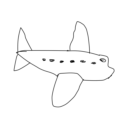
\includegraphics[width=0.5\linewidth]{airplane}
	\caption{Example sketch from the TU Berlin dataset}
	\end{center}
\end{figure}

Eitz et al. ~\cite{eitz2012hdhso} defined a taxonomy of 250 object categories gathered from 20,000 human sketches (TU-Berlin sketch benchmark) from Amazon Mechanical Turk (AMT) from 1,350 participants. This dataset provides diversity in both catergories and sketch styles within classes. The TU- Berlin dataset is currently the largest curated dataset of hand drawn sketches. The dataset has a total of 250 classes, 80 sketches per class, and it is split into three categories: exhaustive, recognizable, and specific. Images within this dataset are available as 1111 x 1111 px PNG files.  An example sketch from this dataset can been see in Figure 2. 

For our project, we first rescaled the original sketches from 1111x1111 px to 128x128 px via bilinear interpolation. Since there are only 80 sketches in each class, we needed to overcome overfitting by performing data augmentation. To augment the training data, we generated additional training sketch examples by horizontally flipping existing training examples as well as inverting all examples to better match the effects of our input dropout. An example of an inverted sketch can be seen in Figure 4. This inversion and horizontal flipping was a similar method in  ~\cite{seddati2015deepsketch} , where they proposed image distortion to improve generalization. The total amount of sketches we had to work with is 40,000. The resized images are then read into memory as grayscale 128x128 arrays.


Even though the database covers a range of object categories, its major shortcoming comes from ambiguous drawn sketches ~\cite{schneider2014sketch}. In order to address this problem, Rosalia et al. ~\cite{schneider2014sketch} were able to find a subset of 160 unambiguous object categories to make a more reliable benchmark. However, we are choosing to use all 250 object categories in order to compare our accuracies with other models. 
 
\begin{figure}[h]
	\begin{center}
	\includegraphics[width=.5\linewidth]{invert_colors_2}
	\caption{Example sketch of inverted with inverted color value that was fed into our model}
	\end{center}
\end{figure}
 

%-------------------------------------------------------------------------

\section{Experiment}

to do: it says you should have a confusion matrix or a roc curve since we're doing classification, but we have so many classes. just throw on in there? thoughts?

also can you make our train and test val graphs bigger/ take up the top half of the page? right now it's squeezed and really small. i wasn't able to do that 

 Our approach follows a fairly standard image classification pipeline. Following previous work we performed 3-fold cross-validation within
this dataset (2 folds for training and 1 for testing). Image arrays are fed into a CNN with the final output being fed to a 250-unit fully connected layer to generate logits for each class. We then apply a softmax loss function to the logits and optimize the loss using the Adam (Adaptive Moment Estimation) algorithm. We chose to use Adam because  it compares favorably to other adaptive learning-method algorithms.

We tried to train multiple deep ResNets varying from x to x layers to see which one performs better on the TU-Berlin dataset. The network with the most layers was the one that performed the best showing that ConvNets are able to learn concepts that are more abstract with the depth of the network. This is important to highlight, because sketches are generally very abstract. All of the CNNs were trained with batch size of 32. 


With varying amount of layers to make the model deeper, we also tried several approaches of dropout to counter overfitting as well as different sizes of width for our filters. A more aggressive dropout of 60 and a lesser aggressive dropout of 25 does not improve our validation accuracy.  We also tried a variation of width for our layers. Using these different parameters, our best model was our Vanilla ResNet. This best performing model can be seen in Figure 2. With this model, we were able to achieve a test accuracy of 65.15, but the other types of parameters fall within this range of accuracy. The results are brought in Table 1. Note: all of our models are trained for the same number of epochs. 

\begin{table}[h]
\begin{center}
\begin{tabular}{|l|c|}
\hline
Method & \% \\
\hline\hline
ResNet-aggro-dropout &  65.3 \\
ResNet Vanilla & 65.15 \\
ResNet Weak Dropout & 65.6\\
ResNet Wide &  65.3\\ 
ResNet  Wide V2 & 63.9\\
ResNet Wider  &  58.8\\
ResNet Widish  & 62.05\\ 
ResNet Widest &  55.8\\
\hline
\end{tabular}
\end{center}
\caption{Validation performance comparison between our different parameters}
\end{table}
{\small
\bibliographystyle{ieee}
\bibliography{milestone}
}

In Table 1 and Figure 7, we compared all of our model's training and validation accuracies. Looking at the training accuaries (Figure 7), we see that there is a rapid increasement of accuracy over the amount of epochs. The Vanilla ResNet architecture increases most rapidly compared to the others models, but the ResNet-Weak-dropout model reaches the same training accuracies as the Vanilla ResNet model. The Canilla ResNet and Weak-dropout ResNet architecture have the highest training accuracy compared to the other models. On the other hand, all our validation accuracies level out near the end of training. There is a drastic drop in the validation accuracy for Widish-ResNet model, but it the accuracy picks back up and ends up within the same range of validation accuracies as the other models. 

The difference between training accuracy and validation accuracy of our models is a good indicator of overfitting. Based on our results, we realized that ResNets are more prone to overfitting. However, these results show that adding a simple shortcut connection can improve the accuracy in the classification task and make the training process much faster, but  the trade of is that residual networks are more prone to over-fitting which is undesirable. Our results also suggest that depth is the largest contributing factor to classification accuracy, with dropout regularization providing minor improvement. Widening layers does not result in noticeable changes, and the need to reduce memory consumption by reducing network depth in fact leads to lower accuracy. 

\begin{table}[h]
\begin{center}
\begin{tabular}{|l|c|}
\hline
Method & \% \\
\hline\hline
SIFT-varient + BoF + SVM  ~\cite{eitz2012hdhso}  &  56 \\
IDM + SVM ~\cite{yesilbek2015svm} & 71.30 \\
ConvNet ~\cite{seddati2015deepsketch}  & 75.42\\
ConvNet ~\cite{seddati2016deepsketch} & 77.69\\
ConvNet -- Ours & 65.15 \\
\hline
\end{tabular}
\end{center}
\caption{Test accuracy comparison of our model versus other methods.}
\end{table}
{\small
\bibliographystyle{ieee}
\bibliography{milestone}
}

Our experiments illustrate the complexity of free-hand sketch recognition. An example of the variability of sketches can be seen in Figure 5. This type of varaibility of sketches causes the model to be confused. Where if some edges are similar to another previous trained edge, it will think that particular sketch will belong to a class that is not its true class. An example of such can be viewed in Figure 6. For Figure 6, the model was presented with the airplane (right), and the model classified it as a syringe (left). Notice how similar the edges are within these two sketches, and there is no "true" airplane wing either which is a distinguishable feature for an airplane. 

Table 2 summarizes the overall performance in terms of average recognition accuracy for various architectures compared to our highest performing model. While our CNN  model?s performance is not quite as strong as the CNN model of [~\cite{krizhevsky2012imagenet}], in terms of test accuracies, we would like to point out that the authors used a larger CNN on a larger external dataset through pooling additional sketches through Google. 



\begin{figure}[h]
	\begin{center}
	\includegraphics[width=1\linewidth]{Spondgebob}
	\caption{ Examples of interclass variations of Spongebob from the TU Berlin dataset highlighting the variability }
	\end{center}
\end{figure}


Though our model was able to outperform the traditional multi-class support vector classifiers (SVMs) [1] , there is still more improvement that can be done. Along with that, we were not able to train the model as long as we would have hoped. If you notice in Figure 7 the validation accuracy for our models has not completely leveled out. An example of an error our model made can be seen in Figure 5. 


\begin{figure}[h]
	\begin{center}
	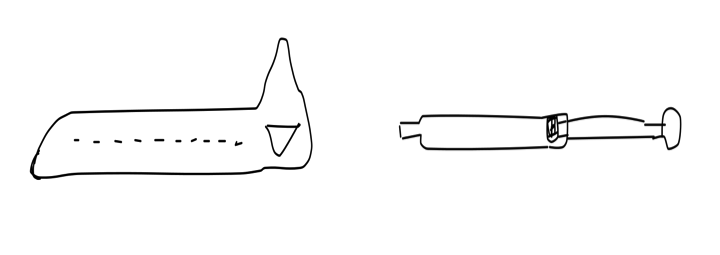
\includegraphics[width=1\linewidth]{mistake}
	\caption{ An example of where our model thought the airplane (right) was a syringe (left). This shows the variability of human sketches }
	\end{center}
\end{figure}


\begin{figure}[h]
	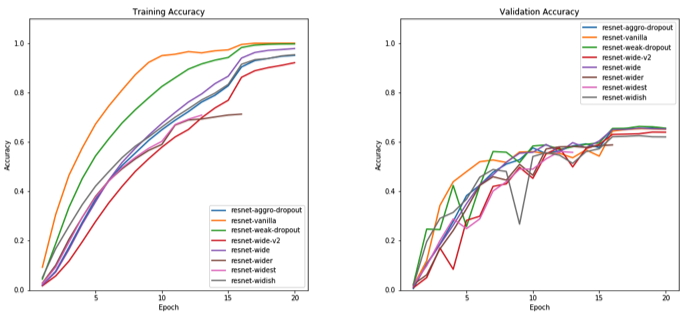
\includegraphics[width=1\linewidth]{train_val}
	\caption{ Training and Validation compairision between all our models  }
	
\end{figure}

%-------------------------------------------------------------------------
\section{Conclusion}

In this paper, we have presented our CNN architecture for freehand sketch recognition. We see that in our model, where free-hand sketches are inherently hard to classify due to large amounts of intraclass variation and interclass overlap, along with a lack of complex visual information, in contrast to traditional image recognition which instead deals with an overabundance of visual information. 
Sketches are usually centered around the edges, and for most neural networks edge detection is within the first few layers. 

Our experiments showed that moderate dropout with deep networks provides the best results. Overaggressive dropout and shallow networks both lead to lower accuracy. Notably, compensating for shallowness with increased width does not result in improved accuracy. 
ResNets are more powerful for very deep networks and and can hurt the performance for shallow networks. ResNets, however, does show promising landscape in deep learning. 

The TU-Berlin dataset, though is the largest, is still relatively limited. However, some things that we can try next is use other networks to train on the TU- Berlin dataset, such as using VGG to train on sketches or the original architecture of ResNet. Our framework source-code and associated data (pre-trained models) can be accessed at: github.com/krinkels/sketch-recognition





\end{document}
